\documentclass[12pt]{thesis} %%%%%%%%%%%%%%%%%%%%%%%%%%%%%%%%%%%%%%%%%%%%%%%%%%
\usepackage[utf8]{inputenc}


\newcommand{\autor}{Vorname Nachname} % Vor und Nachname / GivenName FamilyName (The one on your matriculation)
\newcommand{\matrikel}{123456}	% Matrikel / Matriculation number
\newcommand{\erstgutachter}{Prof. Dr. Frank Steinicke} % Erstgutachter / Primary Reviewer
\newcommand{\zweitgutachter}{Name Zweitgutachter} % Zweitgutachter / Secondary Reviewer
\newcommand{\betreuer}{Name Betreuer} % Betreuer  delete / comment this line if you didn't have a supervisor or the supervior is one of the reviewers
\newcommand{\arbeitstitel}{Tolle Arbeit} % Titel angeben / title of your thesis
\newcommand{\arbeitstyp}{Bachelorarbeit} %Typ angeben / type of the thesis 
\newcommand{\studycourse}{Mensch-Computer-Interaktion} % Sutdiengang/ study course
\newcommand{\german}{ngerman}% delete / comment this line for English

\usepackage{hcisty}
\start{1}{1}
% \start[1]{1} <= show both abstracts
% \start[0]{1} only german. \start[1]{0} only english .\start[0]{0} nothing
% change the abstract.tex and abstractGER.tex to your needs
\newpage\chapter{Kapitelname}\label{chapter:kapitellabel} %%%%%%%%%%%%%%%%%%%%%%%%%%%%
 Itaque earum rerum hic tenetur a sapiente delectus, ut aut reiciendis voluptatibus maiores alias consequatur aut perferendis doloribus asperiores repellat\cite{aho:dragonbook}. See Table ~\ref{table:speedup1} and ~\ref{table:speedup1} and \ref{figure:helloworld}.

\begin{table}[!th]
  \renewcommand{\arraystretch}{1.3}
  \caption{Speed-Up Table I}\label{table:speedup1}
  \vspace{4mm} % hack
  \centering
    \begin{tabular}{|l||r|r|r|}
      \hline      
      program            & basline   & algorithm 1  & alogrithm 2\\
      \hline      
      \hline
      {\tt simple}       &  30 sec   &  20 sec      &  18 sec     \\
      \hline
      {\tt hello world}  &  43 sec   &  27 sec      &  28 sec     \\
      \hline      
    \end{tabular}
\end{table}

\begin{table}[!th]
  \renewcommand{\arraystretch}{1.3}
  \caption{Speed-Up Table II}\label{table:speedup2}
  \vspace{4mm} % hack
  \centering
    \begin{tabular}{|l||r|r|r|}
      \hline      
      program            & basline   & algorithm 1  & alogrithm 2\\
      \hline      
      \hline
      {\tt simple}       &  30 sec   &  20 sec      &  18 sec     \\
      \hline
      {\tt hello world}  &  43 sec   &  27 sec      &  28 sec     \\
      \hline      
    \end{tabular}
\end{table}
Lorem ipsum dolor sit amet, consectetur adipiscing elit, sed do eiusmod tempor incididunt ut labore et dolore magna aliqua. Ut enim ad minim veniam, quis nostrud exercitation ullamco laboris nisi ut aliquip ex ea commodo consequat. Duis aute irure dolor in reprehenderit in voluptate velit esse cillum dolore eu fugiat nulla pariatur. Excepteur sint occaecat cupidatat non proident, sunt in culpa qui officia deserunt mollit anim id est laborum

\begin{figure}[!ht]
\centering
\sourcecode{main.cpp}
\caption{Hello World Program}\label{figure:helloworld}
\end{figure}
Lorem ipsum dolor sit amet, consectetur adipiscing elit, sed do eiusmod tempor incididunt ut labore et dolore magna aliqua. Ut enim ad minim veniam, quis nostrud exercitation ullamco laboris nisi ut aliquip ex ea commodo consequat. Duis aute irure dolor in reprehenderit in voluptate velit esse cillum dolore eu fugiat nulla pariatur. Excepteur sint occaecat cupidatat non proident, sunt in culpa qui officia deserunt mollit anim id est laborum

Lorem ipsum dolor sit amet, consectetur adipiscing elit, sed do eiusmod tempor incididunt ut labore et dolore magna aliqua. Ut enim ad minim veniam, quis nostrud exercitation ullamco laboris nisi ut aliquip ex ea commodo consequat. Duis aute irure dolor in reprehenderit in voluptate velit esse cillum dolore eu fugiat nulla pariatur. Excepteur sint occaecat cupidatat non proident, sunt in culpa qui officia deserunt mollit anim id est laborum

\begin{figure}[!ht] % see https://en.wikibooks.org/wiki/LaTeX/Floats,_Figures_and_Captions for placement parameters
  \centering
  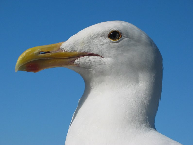
\includegraphics[width=0.5\textwidth]{images/gull.png}
  \caption{A picture of a gull.}
\end{figure}

Lorem ipsum dolor sit amet, consectetur adipiscing elit, sed do eiusmod tempor incididunt ut labore et dolore magna aliqua. Ut enim ad minim veniam, quis nostrud exercitation ullamco laboris nisi ut aliquip ex ea commodo consequat. Duis aute irure dolor in reprehenderit in voluptate velit esse cillum dolore eu fugiat nulla pariatur. Excepteur sint occaecat cupidatat non proident, sunt in culpa qui officia deserunt mollit anim id est laborum

Lorem ipsum dolor sit amet, consectetur adipiscing elit, sed do eiusmod tempor incididunt ut labore et dolore magna aliqua. Ut enim ad minim veniam, quis nostrud exercitation ullamco laboris nisi ut aliquip ex ea commodo consequat. Duis aute irure dolor in reprehenderit in voluptate velit esse cillum dolore eu fugiat nulla pariatur. Excepteur sint occaecat cupidatat non proident, sunt in culpa qui officia deserunt mollit anim id est laborum

Lorem ipsum dolor sit amet, consectetur adipiscing elit, sed do eiusmod tempor incididunt ut labore et dolore magna aliqua. Ut enim ad minim veniam, quis nostrud exercitation ullamco laboris nisi ut aliquip ex ea commodo consequat. 
\begin{figure}[H]
  \centering
  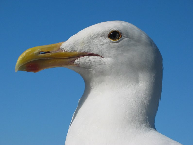
\includegraphics[width=0.5\textwidth]{images/gull.png}
  \caption{A picture of a gull.}
\end{figure}
Duis aute irure dolor in reprehenderit in voluptate velit esse cillum dolore eu fugiat nulla pariatur. Excepteur sint occaecat cupidatat non proident, sunt in culpa qui officia deserunt mollit anim id est laborum

Lorem ipsum dolor sit amet, consectetur adipiscing elit, sed do eiusmod tempor incididunt ut labore et dolore magna aliqua. Ut enim ad minim veniam, quis nostrud exercitation ullamco laboris nisi ut aliquip ex ea commodo consequat. Duis aute irure dolor in reprehenderit in voluptate velit esse cillum dolore eu fugiat nulla pariatur. Excepteur sint occaecat cupidatat non proident, sunt in culpa qui officia deserunt mollit anim id est laborum


% keep an blank line above

\finish